\rfcnumber{0001}
\rfctitle{RFC Lifecycle, Process and Structure}
\rfcdate{October 2025}
\rfcauthor{Qianchen Yu (@QYuQianchen), Tino Breddin (@tolbrino)}
\section{RFC-0001: RFC Lifecycle, Process and
Structure}\label{rfc-0001-rfc-lifecycle-process-and-structure}

\begin{itemize}
\tightlist
\item
  \textbf{RFC Number:} 0001
\item
  \textbf{Title:} RFC Lifecycle, Process and Structure
\item
  \textbf{Status:} Finalised
\item
  \textbf{Author(s):} Qianchen Yu (@QYuQianchen), Tino Breddin
  (@tolbrino)
\item
  \textbf{Created:} 2025-02-20
\item
  \textbf{Updated:} 2025-10-27
\item
  \textbf{Version:} v1.0.0 (Finalised)
\item
  \textbf{Supersedes:} none
\item
  \textbf{Related Links:} none
\end{itemize}

\subsection{1. Abstract}\label{abstract}

This RFC defines the lifecycle, contribution process, versioning system,
governance model, and document structure for RFCs within the HOPR
project. It specifies the stages RFCs progress through, along with the
naming conventions, validation rules, and formatting standards that MUST
be followed to ensure consistency and clarity across all RFC
submissions. The process ensures iterative development with feedback
loops, transparent updates via pull requests (PRs), and clear criteria
for advancing through each stage.

\subsection{2. Motivation}\label{motivation}

The HOPR project requires a clear and consistent process for managing
technical proposals and documenting protocol architecture. A
well-defined lifecycle MUST be established and upheld to maintain
coherence, ensure quality, streamline development, and provide clear
expectations for contributors. This process serves multiple purposes:

\begin{itemize}
\tightlist
\item
  \textbf{Quality assurance}: ensuring that RFCs undergo appropriate
  review and refinement before implementation
\item
  \textbf{Transparency}: making the development process visible and
  accessible to all stakeholders
\item
  \textbf{Version control}: tracking changes and maintaining
  compatibility across protocol versions\\
\item
  \textbf{Coordination}: allowing multiple contributors to work on
  related RFCs without conflicts or inconsistencies
\end{itemize}

\subsection{3. Terminology}\label{terminology}

The key words ``MUST'', ``MUST NOT'', ``REQUIRED'', ``SHALL'', ``SHALL
NOT'', ``SHOULD'', ``SHOULD NOT'', ``RECOMMENDED'', ``MAY'', and
``OPTIONAL'' in this document are to be interpreted as described in
{[}01{]}.

\textbf{Draft}: an RFC is considered a draft from the moment it is
proposed for review. A draft MUST include a clear summary, contextual
background, and initial technical details sufficient for evaluation.
Drafts MUST follow the v0.x.x versioning scheme, with each version being
independently reviewable and, where appropriate, independently
implementable. A draft version (v0.1.0) is assigned as soon as the first
PR is created and the RFC number is allocated.

\subsection{4. Specification}\label{specification}

\subsubsection{4.1. RFC Lifecycle Stages}\label{rfc-lifecycle-stages}

\paragraph{4.1.1. Mermaid Diagram for RFC Lifecycle
Stages}\label{mermaid-diagram-for-rfc-lifecycle-stages}

\begin{figure}
\centering
\pandocbounded{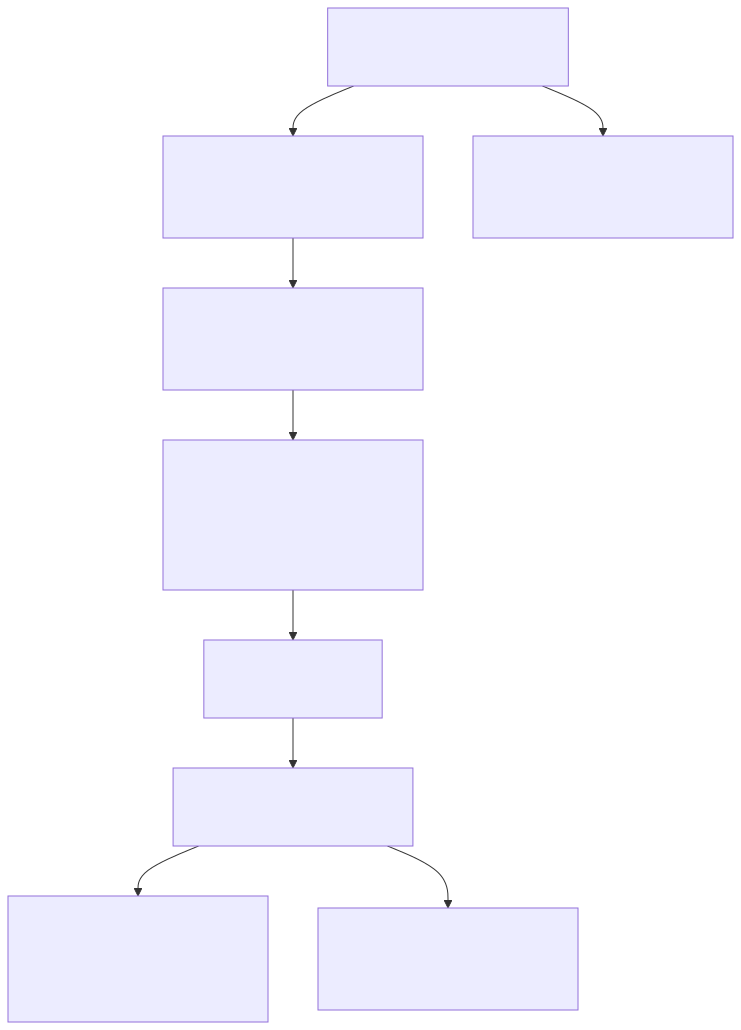
\includegraphics[width=\maxwidth,keepaspectratio,alt={Mermaid Diagram 1}]{0001-rfc-process/mermaid_1.png}}
\caption{Mermaid Diagram 1}
\end{figure}

\paragraph{4.1.2. Stage Descriptions}\label{stage-descriptions}

\begin{itemize}
\tightlist
\item
  \textbf{Raw:} The RFC MUST begin as a raw draft reflecting initial
  ideas. The draft MAY contain incomplete details but MUST provide a
  clear objective.
\item
  \textbf{Discussion:} Upon submission of the initial PR, the RFC number
  and \codebubble{v0.1.0} version are assigned. Feedback SHALL be
  gathered via PRs, with iterative updates reflected in version
  increments \codebubble{(v0.x.x)}.
\item
  \textbf{Review:} The RFC MUST undergo at least one review cycle. The
  draft SHOULD incorporate significant feedback and each iteration MUST
  be independently implementable.
\item
  \textbf{Draft:} The RFC moves into active development and refinement.
  Each update SHALL increment the version (\codebubble{v0.x.x}) to
  indicate progress.
\item
  \textbf{Implementation:} Merging to the main branch signifies
  readiness for practical use, triggering the finalisation process.
\item
  \textbf{Finalised:} The RFC is considered stable and complete, with
  version \codebubble{v1.0.0} assigned. Only errata modifications are
  permitted afterwards.
\item
  \textbf{Errata:} Minor technical corrections post-finalisation MUST be
  documented and result in a patch version increment
  (\codebubble{v1.0.x}). Errata are technical corrections or factual
  updates made after an RFC has been finalised. They MUST NOT alter the
  intended functionality or introduce new features.
\item
  \textbf{Superseded:} Significant updates requiring functionality
  changes MUST be documented in a new RFC, starting at
  \codebubble{v2.0.0} or higher. The original RFC must include
  information that it has been superseded, accompanied by a link to the
  new RFC that supersedes it.
\item
  \textbf{Rejected:} If an RFC does not progress past the discussion
  stage, the reasons MUST be documented.
\end{itemize}

\subsubsection{4.2. File Structure}\label{file-structure}

\begin{codebubbleenv}
RFC-0001-rfc-life-cycle-process/
│
├── 0001-rfc-life-cycle-process.md
├── errata/
│   └── 0001-v1.0.1-erratum.md
└── assets/
    └── life-cycle-overview.png
\end{codebubbleenv}

\begin{center}\rule{0.5\linewidth}{0.5pt}\end{center}

\subsubsection{4.3. Validation Rules}\label{validation-rules}

\begin{itemize}
\tightlist
\item
  The directory MUST be prefixed with uppercased ``RFC'', followed by
  its RFC number, and a succinct title all in lowercase joined by
  hyphens. E.g., \codebubble{RFC-0001-rfc-life-\\ cycle-process}
\item
  The main file MUST be prefixed with its RFC number and a succinct
  title all in lowercase joined by hyphens. E.g.
  \codebubble{0001-rfc-life-cycle-process.md}
\item
  All assets MUST reside in the \codebubble{assets/} folder.
\item
  Errata MUST reside in the \codebubble{errata/} folder.
\end{itemize}

\subsubsection{4.4. RFC Document
Structure}\label{rfc-document-structure}

All RFCs MUST follow a consistent document structure to ensure
readability and maintainability.

\paragraph{4.4.1. Metadata Preface}\label{metadata-preface}

Every RFC MUST begin with the following metadata structure:

\begin{codebubbleenv}
# RFC-XXXX: [Title]

- **RFC Number:** XXXX
- **Title:** [Title in Title Case]
- **Status:** Raw | Discussion | Review | Draft | Implementation | Finalised | Errata | Rejected | Superseded
- **Author(s):** [Name (GitHub Handle)]
- **Created:** YYYY-MM-DD
- **Updated:** YYYY-MM-DD
- **Version:** vX.X.X (Status)
- **Supersedes:** RFC-YYYY (if applicable) | N/A
- **Related Links:** [RFC-XXXX](../RFC-XXXX-[slug]/XXXX-[slug].md) | none
\end{codebubbleenv}

\paragraph{4.4.2. Reference Styles}\label{reference-styles}

RFCs MUST use two distinct reference styles:

\subparagraph{4.4.2.1. RFC-to-RFC
References}\label{rfc-to-rfc-references}

\begin{itemize}
\tightlist
\item
  RFC references to other HOPR RFCs MUST be listed in the metadata's
  \textbf{Related Links:} field
\item
  Format: \codebubble{[RFC-XXXX](../RFC-XXXX-[slug]/XXXX-[slug].md)}
\item
  Multiple references SHALL be separated by commas
\item
  If no RFC references exist, the field MUST contain ``none''
\item
  Example:
  \codebubble{[RFC-0002](../RFC-0002-mixnet-keywords/0002-mixnet-keywords.md), [RFC-0004](../RFC-0004-hopr-packet-protocol/0004-hopr-packet-protocol.md)}
\end{itemize}

\subparagraph{4.4.2.2. External References}\label{external-references}

\begin{itemize}
\item
  External references MUST be listed in a dedicated
  \codebubble{\#\# References} section at the end of the document
\item
  References MUST use sequential numbering with zero-padding: {[}01{]},
  {[}02{]}, etc.
\item
  In-text citations MUST use the numbered format: ``as described in
  {[}01{]}''
\item
  References SHOULD be formatted in accordance with the following style,
  based on APA reference style with numeric labels in square brackets:

  \begin{codebubbleenv}
  [XX] Author(s). (Year). [Title](URL). _Publication_, Volume(Issue), pages.
  \end{codebubbleenv}
\item
  Example:

  \begin{codebubbleenv}
  [01] Chaum, D. (1981). [Untraceable Electronic Mail, Return Addresses, and Digital Pseudonyms](https://www.freehaven.net/anonbib/cache/chaum-mix.pdf). _Communications of the ACM, 24_(2), 84-90.
  \end{codebubbleenv}
\end{itemize}

\paragraph{4.4.3. Required Sections}\label{required-sections}

All RFCs MUST include the following sections:

\begin{enumerate}
\def\labelenumi{\arabic{enumi}.}
\tightlist
\item
  \textbf{Metadata Preface}: A list of information about the RFC and its
  status, as defined in 4.4.1
\item
  \textbf{Abstract}: Brief summary of the RFC's purpose and scope
\item
  \textbf{References}: External citations (if any)
\end{enumerate}

\paragraph{4.4.4. Terminology Formatting
Standards}\label{terminology-formatting-standards}

All RFCs MUST follow consistent terminology formatting to ensure clarity
and professionalism:

\begin{itemize}
\tightlist
\item
  \textbf{Format}: Use bold with colons for term definitions:
  \textbf{Term}: definition
\item
  \textbf{Capitalisation}: Capitalise the first word of each term:
  \textbf{Node}, \textbf{Relay node}, \textbf{Session protocol}
\item
  \textbf{Punctuation}: Always use colons after terms in definition
  lists
\item
  \textbf{Consistency}: Apply the same formatting throughout each RFC
  and across all RFCs
\end{itemize}

Examples: - \textbf{Node}: a process that implements the HOPR protocol
and participates in the mixnet - \textbf{Relay node}: a node that
forwards messages from one node to another in the mixnet -
\textbf{Session protocol}: the protocol layer that provides reliable
message delivery over HOPR packets

Incorrect examples: - \emph{Node}: (should use bold instead of italics)
- \textbf{Node}: (should capitalise first word) - \textbf{Node} (should
include colon) - ``Node'': (should not use quotation marks)

\subsection{5. Design Considerations}\label{design-considerations}

\begin{itemize}
\tightlist
\item
  Modular RFCs SHOULD be preferred
\item
  The PR system MUST be the primary mechanism for contribution, review,
  and errata handling
\end{itemize}

\subsection{6. Compatibility}\label{compatibility}

\begin{itemize}
\tightlist
\item
  New RFCs MUST maintain backward compatibility unless explicitly stated
\item
  Errata MUST NOT introduce backward-incompatible changes
\item
  Breaking changes MUST be reflected in a major version increment
  (\codebubble{v2.0.0})
\end{itemize}

\subsection{7. Security Considerations}\label{security-considerations}

\begin{itemize}
\tightlist
\item
  A security review phase MUST be completed before finalisation
\item
  Errata MUST undergo security review if impacting critical components
\end{itemize}

\subsection{8. Unresolved Questions}\label{unresolved-questions}

\begin{itemize}
\tightlist
\item
  Handling emergency RFCs
\item
  Enforcing cross-RFC dependencies
\item
  Formal approval timeline for errata
\end{itemize}

\subsection{9. Future Work}\label{future-work}

\begin{itemize}
\tightlist
\item
  Automated validation tools
\item
  CI/CD integration for automated versioning and errata checks
\item
  Web interface for publishing RFCs
\end{itemize}

\subsection{10. References}\label{references}

{[}01{]} Bradner, S. (1997).
{Key words for use in RFCs to Indicate Requirement Levels}. \\ \emph{IETF RFC 2119}. \href{https://datatracker.ietf.org/doc/html/rfc2119}{\underline{https://datatracker.ietf.org/doc/html/rfc2119}}

{[}02{]} {RFC Editor Style Guide}. RFC Editor. \href{https://www.rfc-editor.org/styleguide/}{\underline{https://www.rfc-editor.org/styleguide}}

{[}03{]} {Rust RFC Process}. Rust Language Team. \href{https://github.com/rust-lang/rfcs}{\underline{https://github.com/rust-lang/rfcs}}

{[}04{]} {ZeroMQ RFC Process}. ZeroMQ Community. \href{https://rfc.zeromq.org}{\underline{https://rfc.zeromq.org}}

{[}05{]} {VACP2P RFC Index}. Vac Research. \href{https://github.com/vacp2p/rfc-index}{\underline{https://github.com/vacp2p/rfc-index}}